\section{Umsetzung virtueller Spiele in der physischen Welt}

Unter einem virtuellen Spiel verstehen wir jene, die sich ausschlie�lich mit bzw. auf einem Computers spielen lassen. \newline
Es folgen eine Reihe von Spielideen, die in der Welt der virtuellen Spiele sehr popul�r sind und sich f�r die Integration in die physische Welt eignen.
\subsection*{Snake}
Ein absoluter Klassiker, der fr�her auf keinem Handy fehlen durfte. Gerade wegen der Popularit�t und Einfachheit recht interessant es in die physische Welt zu integrieren. In einem begrenzten Areal gilt es eine Schlange geschickt zu steuern. Es m�ssen kleine Items eingesammelt werden, wodurch die Schlange w�chst. Au�erdem muss darauf geachtet werden, dass weder der Rand des Areals noch die eigene Schlange ber�hrt wird.
\newline

\begin{figure}[htbp]
  \centering
    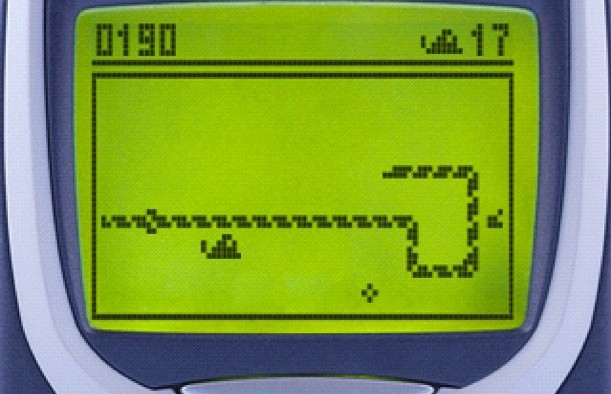
\includegraphics[width=0.5\textwidth]{2-Spielideen/2-1-Umsetzung_virtueller_Spiele_in_der_physischen_Welt/snake.png}
     \caption{Snake auf dem Nokia 3310 
		(Quelle: \url{http://nixtv.de/wp-content/uploads/2014/09/snake.jpg}) }
\end{figure}

Snake ist urspr�nglich ein Einzelspieler-Spiel. Da es un�blich ist, Outdoor-Bewegungsspiele allein zu spielen, haben wir entschieden Snake in der physischen Welt als Mehrspieler-Spiel umzusetzen. \newline Wie wir dies umgesetzt haben, wird sp�ter erl�utert.

\subsection*{Capture the Flag}
Das Spiel ist nicht nur als virtuelles Spiel geeignet, wurde als solches aber erst richtig bekannt. Auch hier ist ein recht einfacher Spielmechanismus ausschlaggebend f�r einen leichten Einsatz in der physischen Welt. Zwei Teams treten gegeneinander an. Jedes Team besitzt eine Basis mit einer Flagge, dessen Standort f�r das gegnerische Team bekannt ist. Es wird versucht die Flagge des jeweils anderen Teams zur eigenen Basis zu bringen. Gelingt dies w�hrend die eigene Flagge nicht vom gegnerischen Team "`entf�hrt"' wurde, wird gepunktet. Wird eine gewisse Punktzahl erreicht, gilt das Spiel als gewonnen.
\newline Hilfreich bei der Integration in die physische Welt w�ren zum einen eine Richtungsangabe der Basis des gegnerischen Teams oder gar eine Karte, auf der die Basis angezeigt wird (eventuell auch die Position der eigenen Flagge, Position der Mitspieler, etc.), zum anderen der aktuelle Punktestand der Teams (eventuell mit Highscore).

\subsection*{Domination}
Meist in Kriegsszenarien integrierter virtueller Spielmodi, der sich mit wenig Aufwand in die physische Welt �bertragen l�sst. Zwei Teams treten gegeneinander an. Jedes Team hat einen Punktestand, der zu Anfang gleich ist, sich aber stetig verringert. Sinkt der Punktestand auf Null, so ist das Spiel f�r dieses Team verloren. Es gibt verschiedene Areale, die eingenommen werden k�nnen. Hat ein Team mehr Areale eingenommen als das Andere, l�uft der Punktestand des Teams, das weniger Areale in besitzt hat, schneller gegen Null.
\newline Verwirklicht werden kann das ganze, indem vor allem der Punktestand umgesetzt wird. Ebenfalls nicht unwichtig ist die Anzeige (z.B. auf einer Karte) der einzunehmenden Areale und in welchem Besitz sie sich gerade befinden. Au�erdem k�nnte dargestellt werden wo sich die eigenen Teammitglieder befinden.